\begin{pastexam}[label={px:ncu-109-dsa-03}]{中央資工所 109 學年度 第 3 題}
（複選；每題 5 分，全對才給分，答錯倒扣 1.25 分）

Given the following binary tree.

\begin{center}
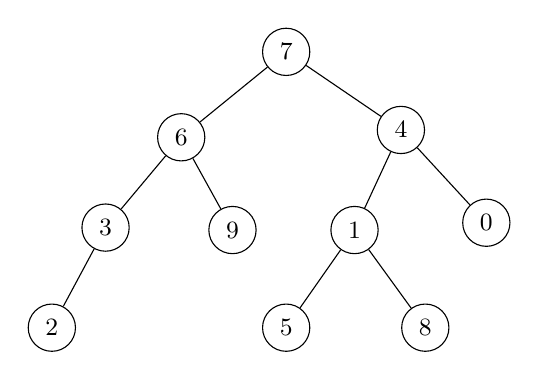
\begin{tikzpicture}[x=0.62cm,y=0.62cm,v/.style={circle,draw,inner sep=1pt,minimum size=6mm,font=\small}]
\node[v] (7) at (5.8,-0.9) {7};
\node[v] (6) at (3.65,-2.65) {6};
\node[v] (4) at (8.15,-2.5) {4};
\node[v] (3) at (2.1,-4.5) {3};
\node[v] (9) at (4.7,-4.55) {9};
\node[v] (1) at (7.2,-4.55) {1};
\node[v] (0) at (9.9,-4.4) {0};
\node[v] (2) at (1.0,-6.55) {2};
\node[v] (5) at (5.8,-6.55) {5};
\node[v] (8) at (8.65,-6.55) {8};
\draw (7)--(6) (7)--(4) (6)--(3) (6)--(9) (4)--(1) (4)--(0) (3)--(2) (1)--(5) (1)--(8);
\end{tikzpicture}
\end{center}

If we make this binary tree a threaded binary tree, what nodes are pointed by threads of node 3?\\
(A)~node 6 \qquad (B)~node 2 \qquad (C)~node 7 \qquad (D)~node 9
\end{pastexam}

\begin{pastsoln}
答案：(A)。

題目沒有說是哪一種引線，一般說的引線二元樹是\textbf{中序引線}（資結書第~7.5~節）：左指標原本是
\NIL 的，改指中序的前一個節點；右指標原本是 \NIL 的，改指中序的下一個節點。 有子節點的那一邊仍然
指向子節點，不是引線。

這棵樹的中序走訪：
\[
2,\ 3,\ 6,\ 9,\ 7,\ 5,\ 1,\ 8,\ 4,\ 0.
\]
（左子樹 $6$ 的中序是 $2, 3, 6, 9$，接著根 $7$，右子樹 $4$ 的中序是 $5, 1, 8, 4, 0$。）

節點 $3$ 的左子節點是 $2$，所以左指標是一般的指標，不是引線；右指標原本是 \NIL，變成引線，指向
中序裡 $3$ 的下一個節點 $6$。 節點 $3$ 只有一條引線，指向 $6$，選 (A)。

逐項看：
\begin{itemize}
\item (A) node 6：$3$ 的右引線指向它，對。
\item (B) node 2：$2$ 是 $3$ 的左子節點，那是原本的指標，不是引線。 錯。
\item (C) node 7：$7$ 在中序裡和 $3$ 不相鄰，沒有引線指向它。 錯。
\item (D) node 9：$9$ 是 $6$ 的右子節點，中序在 $6$ 後面，和 $3$ 無關。 錯。
\end{itemize}
如果改成前序或後序引線，$3$ 的右引線會指向前序的下一個 $2$ 或後序的下一個 $9$，答案就不同了；
題目沒有特別說明，照慣例用中序。
\end{pastsoln}
